% (find-LATEX "2021-1-C2-somas-2.tex")
% (defun c () (interactive) (find-LATEXsh "lualatex -record 2021-1-C2-somas-2.tex" :end))
% (defun C () (interactive) (find-LATEXsh "lualatex 2021-1-C2-somas-2.tex" "Success!!!"))
% (defun D () (interactive) (find-pdf-page      "~/LATEX/2021-1-C2-somas-2.pdf"))
% (defun d () (interactive) (find-pdftools-page "~/LATEX/2021-1-C2-somas-2.pdf"))
% (defun e () (interactive) (find-LATEX "2021-1-C2-somas-2.tex"))
% (defun o () (interactive) (find-LATEX "2020-2-C2-somas-2.tex"))
% (defun u () (interactive) (find-latex-upload-links "2021-1-C2-somas-2"))
% (defun v () (interactive) (find-2a '(e) '(d)))
% (defun d0 () (interactive) (find-ebuffer "2021-1-C2-somas-2.pdf"))
% (defun cv () (interactive) (C) (ee-kill-this-buffer) (v) (g))
%          (code-eec-LATEX "2021-1-C2-somas-2")
% (find-pdf-page   "~/LATEX/2021-1-C2-somas-2.pdf")
% (find-sh0 "cp -v  ~/LATEX/2021-1-C2-somas-2.pdf /tmp/")
% (find-sh0 "cp -v  ~/LATEX/2021-1-C2-somas-2.pdf /tmp/pen/")
%     (find-xournalpp "/tmp/2021-1-C2-somas-2.pdf")
%   file:///home/edrx/LATEX/2021-1-C2-somas-2.pdf
%               file:///tmp/2021-1-C2-somas-2.pdf
%           file:///tmp/pen/2021-1-C2-somas-2.pdf
% http://angg.twu.net/LATEX/2021-1-C2-somas-2.pdf
% (find-LATEX "2019.mk")
% (find-CN-aula-links "2021-1-C2-somas-2" "2" "c2m211somas2" "c2so2")

% «.video-1»			(to "video-1")
% «.video-2»			(to "video-2")
%
% «.defs»			(to "defs")
% «.title»			(to "title")
% «.hernandez»			(to "hernandez")
%
% «.porque-aprender-isto»	(to "porque-aprender-isto")
% «.um-milhao-de-pontos»	(to "um-milhao-de-pontos")
% «.imagens-de-conjuntos»	(to "imagens-de-conjuntos")
% «.exercicio-1»		(to "exercicio-1")
% «.imagens-de-intervalos»	(to "imagens-de-intervalos")
% «.exercicio-2»		(to "exercicio-2")
% «.tipos»			(to "tipos")
% «.exercicio-3»		(to "exercicio-3")
% «.exercicio-4»		(to "exercicio-4")
% «.exercicio-4-cont»		(to "exercicio-4-cont")
% «.exercicio-4f-dica»		(to "exercicio-4f-dica")
% «.exercicio-5»		(to "exercicio-5")
% «.exercicio-6»		(to "exercicio-6")
% «.exercicio-7»		(to "exercicio-7")
% «.exercicio-7-figura»		(to "exercicio-7-figura")
% «.dois-jeitos-imagens»	(to "dois-jeitos-imagens")
% «.sups-e-infs-em-portugues»	(to "sups-e-infs-em-portugues")
% «.exercicio-8»		(to "exercicio-8")
% «.exercicio-9»		(to "exercicio-9")
% «.exercicio-10»		(to "exercicio-10")
% «.exercicio-11»		(to "exercicio-11")
% «.metodos-nomes»		(to "metodos-nomes")
% «.metodos-nomes-2»		(to "metodos-nomes-2")
% «.exercicio-12»		(to "exercicio-12")
% «.exercicio-13»		(to "exercicio-13")
% «.exercicio-14»		(to "exercicio-14")
% «.definicao-integral»		(to "definicao-integral")
% «.intoverunder»		(to "intoverunder")
% «.exercicio-15»		(to "exercicio-15")
% «.exercicio-16»		(to "exercicio-16")
% «.exercicio-16-defs»		(to "exercicio-16-defs")
% «.exercicio-16-fig1»		(to "exercicio-16-fig1")
% «.exercicio-16-fig2»		(to "exercicio-16-fig2")
% «.exercicio-17»		(to "exercicio-17")
% «.claramente-integravel»	(to "claramente-integravel")
% «.claramente-integravel-2»	(to "claramente-integravel-2")
% «.claramente-integravel-3»	(to "claramente-integravel-3")
% «.claramente-integravel-p»	(to "claramente-integravel-p")
% «.funcoes-escada»		(to "funcoes-escada")
% «.exercicio-18»		(to "exercicio-18")
% «.dirichlet»			(to "dirichlet")
% «.dirichlet-2»		(to "dirichlet-2")
% «.dirichlet-3»		(to "dirichlet-3")
% «.exercicio-19»		(to "exercicio-19")
% «.trailer»			(to "trailer")
%
% «.djvuize»	(to "djvuize")



% Video:
% «video-1»  (to ".video-1")
% (c2m211somas2a  "video-1")
% (find-ssr-links     "c2m211somas2" "2021-1-C2-somas-2" "qR6M2U_eiwE")
% (code-eevvideo      "c2m211somas2" "2021-1-C2-somas-2" "qR6M2U_eiwE")
% (code-eevlinksvideo "c2m211somas2" "2021-1-C2-somas-2" "qR6M2U_eiwE")
% (find-c2m211somas2video "0:00")
% (find-c2m211somas2video "2:23" "Exercício 3: Tipos")
% (find-c2m211somas2video "3:39" "Exercício 3: tipos")
% (find-c2m211somas2video "6:29" "alguns slides sobre somatórios")
%
% «video-2»  (to ".video-2")
% (c2m211somas2a  "video-2")
% (find-ssr-links     "c2m211somas2" "2021-1-C2-somas-2b" "ZOAJ8wLnFn8")
% (code-eevvideo      "c2m211somas2" "2021-1-C2-somas-2b" "ZOAJ8wLnFn8")
% (code-eevlinksvideo "c2m211somas2" "2021-1-C2-somas-2b" "ZOAJ8wLnFn8")
% (find-c2m211somas2video "0:00" "28/jul/2021")
% (find-c2m211somas2video "0:17" "miniteste exercicio 12")
% (find-c2m211somas2video "0:28" "miniteste exercicio 14")
% (find-c2m211somas2video "0:40" "conseguiam enxergar todos os máximos e mínimos")
% (find-c2m211somas2video "0:45" "[max] e [min] nem sempre")
% (find-c2m211somas2video "1:05" "enquanto o [sup] daria isso aqui")
% (find-c2m211somas2video "2:25" "identificarem essas expressões nos desenhos")
% (find-c2m211somas2video "2:45" "nem sempre eu escolhi as melhores cores")
% (find-c2m211somas2video "3:07" "entre as duas aproximações")
% (find-c2m211somas2video "3:52" "se vocês entenderem esses retângulos como áreas")
% (find-c2m211somas2video "4:41" "6(6-2) + 4(10-6)")
% (find-c2m211somas2video "5:09" "quando a gente conseguir entender essas desigualdades")
% (find-c2m211somas2video "5:22" "no semestre passado")
% (find-c2m211somas2video "5:35" "na P1")
% (find-c2m211somas2video "5:47" "contando quadradinhos - inclusive exercício")
% (find-c2m211somas2video "6:23" "se vocês não conseguirem calcular no olho")
% (find-c2m211somas2video "6:40" "eu dei uma questão em que eu não dava o desenho")

% Videos antigos:
% (c2m202somas2a "video-1-imagens")
% (c2m202somas2a "video-2-infs-e-sups")



\documentclass[oneside,12pt]{article}
\usepackage[colorlinks,citecolor=DarkRed,urlcolor=DarkRed]{hyperref} % (find-es "tex" "hyperref")
\usepackage{amsmath}
\usepackage{amsfonts}
\usepackage{amssymb}
\usepackage{pict2e}
\usepackage[x11names,svgnames]{xcolor} % (find-es "tex" "xcolor")
\usepackage{colorweb}                  % (find-es "tex" "colorweb")
%\usepackage{tikz}
%
% (find-dn6 "preamble6.lua" "preamble0")
%\usepackage{proof}   % For derivation trees ("%:" lines)
%\input diagxy        % For 2D diagrams ("%D" lines)
%\xyoption{curve}     % For the ".curve=" feature in 2D diagrams
%
%\usepackage{edrx15}               % (find-LATEX "edrx15.sty")
\usepackage{edrx21}               % (find-LATEX "edrx21.sty")
\input edrxaccents.tex            % (find-LATEX "edrxaccents.tex")
\input edrxchars.tex              % (find-LATEX "edrxchars.tex")
\input edrxheadfoot.tex           % (find-LATEX "edrxheadfoot.tex")
\input edrxgac2.tex               % (find-LATEX "edrxgac2.tex")
%
%\usepackage[backend=biber,
%   style=alphabetic]{biblatex}            % (find-es "tex" "biber")
%\addbibresource{catsem-slides.bib}        % (find-LATEX "catsem-slides.bib")
%
% (find-es "tex" "geometry")
\usepackage[a6paper, landscape,
            top=1.5cm, bottom=.25cm, left=1cm, right=1cm, includefoot
           ]{geometry}
%
\begin{document}

\catcode`\^^J=10
\directlua{dofile "dednat6load.lua"}  % (find-LATEX "dednat6load.lua")

%L dofile "edrxtikz.lua"  -- (find-LATEX "edrxtikz.lua")
%L dofile "edrxpict.lua"  -- (find-LATEX "edrxpict.lua")
\pu

% «defs»  (to ".defs")
% (find-LATEX "edrx15.sty" "colors-2019")
\long\def\ColorRed   #1{{\color{Red1}#1}}
\long\def\ColorViolet#1{{\color{MagentaVioletLight}#1}}
\long\def\ColorViolet#1{{\color{Violet!50!black}#1}}
\long\def\ColorGreen #1{{\color{SpringDarkHard}#1}}
\long\def\ColorGreen #1{{\color{SpringGreenDark}#1}}
\long\def\ColorGreen #1{{\color{SpringGreen4}#1}}
\long\def\ColorGray  #1{{\color{GrayLight}#1}}
\long\def\ColorGray  #1{{\color{black!30!white}#1}}
\long\def\ColorBrown #1{{\color{Brown}#1}}
\long\def\ColorBrown #1{{\color{brown}#1}}
\long\def\ColorOrange#1{{\color{orange}#1}}

\long\def\ColorShort #1{{\color{SpringGreen4}#1}}
\long\def\ColorLong  #1{{\color{Red1}#1}}

\def\frown{\ensuremath{{=}{(}}}
\def\True {\mathbf{V}}
\def\False{\mathbf{F}}
\def\D    {\displaystyle}

\def\gr   {\mathsf{gr}}
\def\dom  {\mathsf{dom}}
\def\im   {\mathsf{im}}

\def\pmt         #1{\pmat{\text{#1}}}
\def\pmtt      #1#2{\pmat{\text{#1} \\ \text{#2}}}
\def\pmttt   #1#2#3{\pmat{\text{#1} \\ \text{#2} \\ \text{#3}}}
\def\pmtttt#1#2#3#4{\pmat{\text{#1} \\ \text{#2} \\ \text{#3} \\ \text{#4}}}

\def\smt         #1{\sm{\text{#1}}}
\def\smtt      #1#2{\sm{\text{#1} \\ \text{#2}}}
\def\smttt   #1#2#3{\sm{\text{#1} \\ \text{#2} \\ \text{#3}}}
\def\smtttt#1#2#3#4{\sm{\text{#1} \\ \text{#2} \\ \text{#3} \\ \text{#4}}}

\def\drafturl{http://angg.twu.net/LATEX/2021-1-C2.pdf}
\def\drafturl{http://angg.twu.net/2021.1-C2.html}
\def\draftfooter{\tiny \href{\drafturl}{\jobname{}} \ColorBrown{\shorttoday{} \hours}}

\def\inftys {\{-∞,+∞\}}
\def\Rest{\R∪\{-∞,+∞\}}

\def\Intover     #1#2{\overline {∫}_{#1}#2\,dx}
\def\Intunder    #1#2{\underline{∫}_{#1}#2\,dx}
\def\Intoverunder#1#2{\Intover{#1}{#2} - \Intunder{#1}{#2}}

\def\Intxover     #1#2#3{\overline {∫}_{x=#1}^{x=#2}#3\,dx}
\def\Intxunder    #1#2#3{\underline{∫}_{x=#1}^{x=#2}#3\,dx}

\def\Intoverunder   #1#2{\overline{\underline{∫}}_{#1}      #2\,dx}
\def\Intxoverunder#1#2#3{\overline{\underline{∫}}_{x=#1}^{x=#2} #3\,dx}


%  _____ _ _   _                               
% |_   _(_) |_| | ___   _ __   __ _  __ _  ___ 
%   | | | | __| |/ _ \ | '_ \ / _` |/ _` |/ _ \
%   | | | | |_| |  __/ | |_) | (_| | (_| |  __/
%   |_| |_|\__|_|\___| | .__/ \__,_|\__, |\___|
%                      |_|          |___/      
%
% «title»  (to ".title")
% (c2m211somas2p 1 "title")
% (c2m211somas2a   "title")

\thispagestyle{empty}

\begin{center}

\vspace*{1.2cm}

{\bf \Large Cálculo 2 - 2021.1}

\bsk

Aula 4: integrais como somas de retângulos (2)

\bsk

Eduardo Ochs - RCN/PURO/UFF

\url{http://angg.twu.net/2021.1-C2.html}

\end{center}

\newpage

% «hernandez»  (to ".hernandez")
% (c2m211somas2p 2 "hernandez")
% (c2m211somas2a   "hernandez")

{\bf Aproximações por cima e por baixo}

Uma das figuras na p.2 das notas da Cristiane Hernández é esta:

% (find-books "__analysis/__analysis.el" "hernandez")
% (find-c2crishernandezpage (+ 10  2) "")
% (find-latexgimp-links "2020-1-C2/area-hernandez-1")

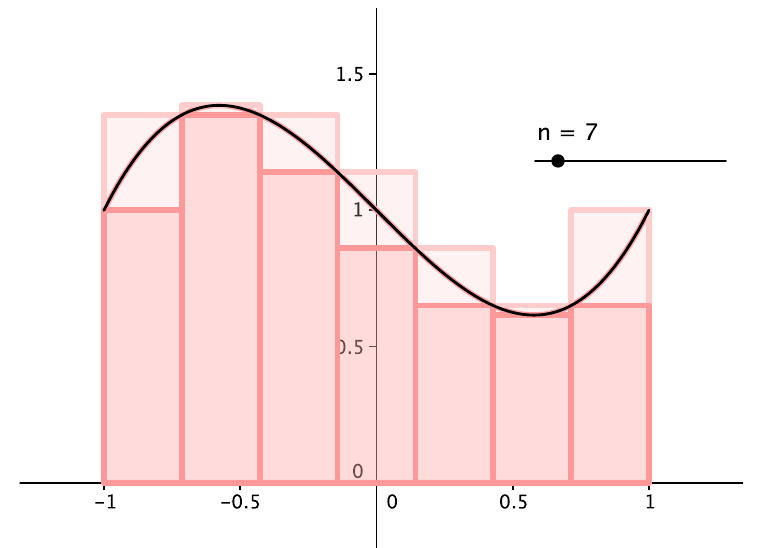
\includegraphics[width=6cm]{2020-1-C2/area-hernandez-1.png}

Ela mostra uma tentativa de calcular uma integral fazendo uma {\sl
  aproximação por retângulos por baixo} e uma {\sl aproximação por
  retângulos por cima} para $y=f(x)$ no intervalo entre $x=-1$ e
$x=1$. A curva $y=f(x)$ fica entre estas duas aproximações.

\newpage

% «porque-aprender-isto»  (to ".porque-aprender-isto")
% (c2m211somas2p 3 "porque-aprender-isto")
% (c2m211somas2a   "porque-aprender-isto")

{\bf Porque aprender isto}

\ssk

As definições {\sl formais} de ``aproximação por retângulos por
baixo'' e ``aproximação por retângulos por cima'' são bem trabalhosas.
Elas envolvem alguns truques com conjuntos infinitos, ``para todo'' e
``existe'', que a maioria dos livros de Cálculo pula...

Nós vamos ver essas definições em detalhes porque entendê-las e
aprender a visualizar cada subexpressão delas vai acabar sendo
\ColorRed{muito} útil pras próximas matérias de Matemática do curso de
vocês.

No material da aula 2 eu pedi pra vocês aprenderem a fazer certos
desenhos sem contas, chamei isso de o ``jeito esperto'', e disse que
fazê-los calculando todas as coordenadas era o ``jeito burro''. Na
discussão desse material pelo Telegram a Eduarda me pediu pra explicar
melhor isso, e eu dei essa explicação aqui...

\newpage

% «um-milhao-de-pontos»  (to ".um-milhao-de-pontos")
% (c2m211somas2p 4 "um-milhao-de-pontos")
% (c2m211somas2a   "um-milhao-de-pontos")

Tenta aprender a não fazer as contas... se você fizer tudo pelas
contas você vai demorar muito mais e não vai descobrir um monte de
truques importantes que a gente só descobre se a gente tenta aprender
a visualizar tudo geometricamente...

Acho que eu tenho um exemplo bom.

Num dos primeiros slides eu usei uma figura copiada das notas da
Cristiane Hernandez em que ela usa uma partição com 7 intervalos - ela
até escreveu do lado ``$n=7$''...

Daqui a pouco a gente vai ter que usar figuras --- que a gente não vai
poder desenhar explicitamente com todos os detalhes --- com 10
intervalos, ou 100, ou 1000, ou um milhão de intervalos

Se você aprender a visualizar tudo sem contas você vai conseguir
visualizar a figura com um milhão de intervalos em poucos segundos.

E se você tiver que fazer as contas pra um milhão de intervalos você
vai gastar um tempo que a gente não tem $\frown$



\newpage

% «imagens-de-conjuntos»  (to ".imagens-de-conjuntos")
% (c2m211somas2p 5 "imagens-de-conjuntos")
% (c2m211somas2a   "imagens-de-conjuntos")

{\bf Imagens de conjuntos}

\ssk

Dê uma olhada na seção 1.3 do Martins/Martins.

% (find-martinscdipage (+ 10  18) "1.3 Grafico de uma funcao")

Nós vamos usar uma notação um pouco diferente da deles.

Se $f:A→\R$ (obs: $A=\dom(f)$),
%
$$\begin{array}{rcl}
  \gr_f    &=& \setofst{(x,f(x))}{x∈A}, \\
  \im_f    &=& \setofst{f(x)}{x∈A}, \\
  \gr_f(B) &=& \setofst{(x,f(x))}{x∈B}, \\
  F(B)     &=& \setofst{f(x)}{x∈B}, \\
  \end{array}
$$

\newpage

Por exemplo, se
%
$$\begin{array}{rrcl}
  f: & \R &\to& \R \\
     &  x &↦&   x^2 \\
  \end{array}
$$

e $B=\{-1,0,1,2\}$ então:
%
$$\begin{array}{rcl}
  \gr_f(B) &=& \gr_f(\{-1,0,1,2\}), \\
           &=& \setofst{(x,f(x))}{x∈\{-1,0,1,2\}} \\
           &=& \{(-1,f(-1)), (0,f(0)), (1,f(1)), (2,f(2))\} \\
           &=& \{(-1,(-1)^2), (0,0^2), (1,1^2), (2,2^2)\} \\
           &=& \{(-1,1), (0,0), (1,1), (2,4)\} \\[5pt]
  F(B)     &=& \setofst{f(x)}{x∈\{-1,0,1,2\}} \\
           &=& \{(-1)^2, 0^2, 1^2, 2^2\} \\
           &=& \{1, 0, 1, 4\} \\
           &=& \{0, 1, 4\} \\
  \end{array}
$$


\newpage

% «exercicio-1»  (to ".exercicio-1")
% (c2m211somas2p 7 "exercicio-1")
% (c2m211somas2a   "exercicio-1")

Se visualizarmos $B$ como um subconjunto do eixo $x$

então $\gr_f(B)$ é o resultado de ``levantar'' cada ponto de $B$

para o ponto correspondente no gráfico de $f$,

e $F(B)$ é o resultado de projetar todos os pontos de $\gr_f(B)$

no eixo $y$.

\msk

{\bf Exercício 1.}

Sejam $f(x)=x^2$ e $B=\{\ColorRed{-3},\ColorRed{-2},-1,0,1,2\}$.

a) Calcule $F(B)$.

b) Calcule $\gr_f(B)$.

c) Represente graficamente num gráfico só: $B$ ``como um subconjunto
do eixo $x$'', $\gr_f(B)$, $F(B)$ ``como um subconjunto do eixo $y$''.

d) Represente graficamente num (outro) gráfico só: $B$ ``como um
subconjunto do eixo $\ColorRed{y}$'', $\gr_f(B)$, $F(B)$ ``como um
subconjunto do eixo $\ColorRed{y}$''.

% Pra representar o conjunto {-3,-2,-1,0,1,2} no eixo x você vai pôr bolinhas nestes pontos do R^2:
% {(-3,0),(-2,0),(-1,0),(0,0),(1,0),(2,0)}

% Pra representar o conjunto {-3,-2,-1,0,1,2} no eixo y você vai pôr bolinhas nestes pontos do R^2:
% {(0,-3),(0,-2),(0,-1),(0,0),(0,1),(0,2)}


\newpage

% «imagens-de-intervalos»  (to ".imagens-de-intervalos")
% (c2m211somas2p 8 "imagens-de-intervalos")
% (c2m211somas2a   "imagens-de-intervalos")

{\bf Imagens de intervalos}

\ssk

% (find-LATEX "edrxpict.lua" "beginpicture")

Seja:

$f(x)=
    \unitlength=10pt
    \celllower=2.5pt%
    \def\cellfont{\scriptsize}%
    %
    \vcenter{\hbox{%
    \beginpicture(0,0)(11,7)
    \pictgrid%
    \pictpiecewise{(0,3)--(3,6)--(8,1)--(11,4)}%
    \put(3,6.5){\cell{(3,6)}}%
    \put(8,0.5){\cell{(8,1)}}%
    \pictaxes%
    \end{picture}%
    }}
    =
    \scalebox{1.0}{$
    \begin{cases}
    x+3 & \text{quando $x≤3$}, \\
    9-x & \text{quando $3<x<8$}, \\
    x-7 & \text{quando $8≤x$} \\
    \end{cases}
    $}
   $

\bsk


Se $B$ é um conjunto infinito ---

por exemplo, $B = [1,2) ∪ [6,7)$ ---

não dá pra calcularmos $\gr_f(B)$ e $F(B)$

fazendo as contas pra todos os pontos...

É melhor fazer desenhos.







\newpage

\phantom{a}

\vspace*{-1cm}

$%f(x)=
    \unitlength=25pt
    \celllower=2.5pt%
    \def\cellfont{\scriptsize}%
    %
    \vcenter{\hbox{%
    \beginpicture(0,0)(11,7)
    \pictgrid%
    \pictpiecewise{(0,3)--(3,6)--(8,1)--(11,4)}%
    \put(3,6.25){\cell{(3,6)}}%
    \put(8,0.75){\cell{(8,1)}}%
    \pictaxes%
    \ColorOrange{%
      %\linethickness{4pt}
      \pictpiecewise{(1,0)c--(2,0)o
                     (1,4)c--(2,5)o
                     (0,4)c--(0,5)o
                     (6,0)c--(7,0)o
                     (6,3)c--(7,2)o
                     (0,3)c--(0,2)o
                    }%
    }
    \end{picture}%
    }}
   $

\bsk

Neste caso temos

$F([1,2) ∪ [6,7)) = (2,3] ∪ [4,5)$.


\newpage

% «exercicio-2»  (to ".exercicio-2")
% (c2m211somas2p 10 "exercicio-2")
% (c2m211somas2a    "exercicio-2")

{\bf Exercício 2.}

Seja $f$ a função definida dois slides atrás.

Calcule:

a) $F([2,3))$

b) $F([2,4))$

c) $F((2,4))$

d) $F((2,9))$

e) $F([1,2)∪[4,5))$

f) $F([1,2)∪\{3\}∪[4,5))$

\msk

\newpage

% «tipos»  (to ".tipos")
% (c2m211somas2p 11 "tipos")
% (c2m211somas2a    "tipos")
% Orig: (c3m211vlp 3 "tipos")
%       (c3m211vla   "tipos")

{\bf Tipos}

\ssk

Tudo que nós vamos fazer \ColorRed{neste PDF} pode ser {\sl
  visualizado} e {\sl tipado}. Você já viu um pouco de tipos em {\tt
  C} e em Física; em Física os ``tipos'' são parcialmente determinados
pelas unidades --- metros são distância, segundos são tempo,
metros/segundo é uma unidade de velocidade, e assim por diante...

% (find-bortolossi5page (+ -162 164) "5.2. Definições e exemplos")
% (find-bortolossi5page (+ -162 165)   "Fig. 5.2: Interpretação geométrica")

Nos itens c e d do exercício 1 você viu que você podia interpretar $B$
como um subconjunto do eixo $x$ e $F(B)$ como subconjunto do eixo $y$
e também podia tentar fazer o contrário --- $B$ como subconjunto do
eixo $y$ e $F(B)$ como subconjunto do eixo $x$ --- mas a primeira
interpretação fazia muito mais sentido.

\newpage

% «exercicio-3»  (to ".exercicio-3")
% (c2m211somas2p 11 "exercicio-3")
% (c2m211somas2a    "exercicio-3")

{\bf Exercício 3.}

Para cada uma dos proposições abaixo diga

se ela é verdadeira ou falsa.

a) $∀x∈[7,9]. \, 1<f(x)$

b) $∀x∈[7,9]. \, 1≤f(x)$

c) $∃x∈[7,9]. \, 1<f(x)$

d) $∃x∈[7,9]. \, 1≤f(x)$


\msk

Dica:

\def\pex{\smtt{ponto no}{eixo $x$}}
\def\pey{\smtt{ponto no}{eixo $y$}}
\def\iex{\smtt{intervalo}{no eixo $x$}}
\def\iey{\smtt{intervalo}{no eixo $y$}}
\def\sex{\smtt{subconjunto}{do eixo $x$}}
\def\sey{\smtt{subconjunto}{do eixo $y$}}

\def\und#1#2{\underbrace{#1}_{#2}}
\def\upex #1{\underbrace{#1}_{\pex}}
\def\upey #1{\underbrace{#1}_{\pey}}
\def\uiex #1{\underbrace{#1}_{\iex}}
\def\uiey #1{\underbrace{#1}_{\iey}}
\def\usex #1{\underbrace{#1}_{\sex}}
\def\usey #1{\underbrace{#1}_{\sey}}
\def\ubool#1{\underbrace{#1}_{\text{bool}}}

$\ubool{∀ \upex{x} ∈ \usex{[7,9]}. \, \ubool{\upey{1} < \upey{f(\upex{x})}}}$

\newpage

% «exercicio-4»  (to ".exercicio-4")
% (c2m211somas2p 13 "exercicio-4")
% (c2m211somas2a    "exercicio-4")


Da mesma forma que podemos definir funções

nós podemos definir proposições.

Uma proposição é uma função que retorna $\True$ ou $\False$.

Seja $P(y) = (∀x∈[7,9]. \, y≤f(x))$,

onde esta função $f$ é a do slide 8.

\msk

{\bf Exercício 4 (obs: difícil! Veja abaixo...)}

Para cada uma das proposições abaixo

diga se ela é verdadeira ou falsa.

a) $P(0.5)$ 

b) $P(0.99)$ 

c) $P(1)$ 

d) $P(1.01)$ 

e) $P(2)$ 

\msk

Se você tiver dificuldade comece pelos itens do próximo slide.



\newpage

% «exercicio-4-cont»  (to ".exercicio-4-cont")
% (c2m211somas2p 14 "exercicio-4-cont")
% (c2m211somas2a    "exercicio-4-cont")
% (c2m211substp 23 "para-todo-e-existe")
% (c2m211substa    "para-todo-e-existe")

{\bf Exercício 4 (cont.)}

\ssk

Sejam $f$ a função do slide 8, e:
%
$$\begin{array}{rcl}
  G(x,y) &=& (y≤f(x)) \\
    Q(y) &=& (∀x∈\{7,8,9\}. \, y≤f(x)) \\
         &=& (∀x∈\{7,8,9\}. \, G(x,y)) \\
  \end{array}
$$

f) Calcule $G(7,2)$, $G(8,2)$, $G(9,2)$. 

g) Calcule $G(7,1)$, $G(8,1)$, $G(9,1)$. 

h) Use as idéias dos slides 23--26 do PDF sobre o `$[:=]$'

pra representar o que você obteve nos itens (f) e (g) como

bolinhas pretas e brancas nos pontos $(7,2)$, $(8,2)$, $(9,2)$,

$(7,1)$, $(8,1)$ e $(9,1)$ do plano $xy$. Link:

\msk

% http://angg.twu.net/LATEX/2021-1-C2-subst.pdf#page=23
% http://angg.twu.net/LATEX/2021-1-C2-subst.pdf#page=26

{\footnotesize

\url{http://angg.twu.net/LATEX/2021-1-C2-subst.pdf\#page=23}

}

\msk



\newpage

{\bf Exercício 4 (cont.)}

\ssk

i) $Q(2)$ corresponde ao `$∧$' de quais três bolinhas? Faça um círculo

(amassado) em torno delas e mande foto pro grupo.

j) $Q(1)$ corresponde ao `$∧$' de quais três bolinhas? Faça um círculo

(amassado) em torno delas e mande foto pro grupo.

\bsk

Expanda e calcule/simplificar cada uma das expressões

abaixo \ColorRed{até onde der}:

\ssk

k) $Q(y)$

l) $Q(0)$

m) $Q(4)$

n) $Q(1.5)$

\msk

Repare que aqui estamos usando o conjunto $\{7,8,9\}$, que

é finito... nos itens a, b, c, d usamos $[7,9]$, que é infinito.

\newpage

% «exercicio-4f-dica»  (to ".exercicio-4f-dica")
% (c2m211somas2p 15 "exercicio-4f-dica")
% (c2m211somas2a    "exercicio-4f-dica")

{\bf Exercício 4: mais dicas}

\ssk

{\bf Dica pro 4k:}

$$\begin{array}{rcl}
              Q(y) &=& (∀x∈\{7,8,9\}. \, y≤f(x)) \\[5pt]
  \text{4k) } Q(y) &=& (y≤f(x))[x:=7] \\
                    &∧& (y≤f(x))[x:=8] \\
                    &∧& (y≤f(x))[x:=9] \\
                   &=& (y≤f(7)) ∧ (y≤f(8)) ∧ (y≤f(9)) \\
                   &=& (y≤2) ∧ (y≤1) ∧ (y≤2) \\
  \end{array}
$$


\bsk
\msk

{\bf ``Comentários sobre o exercício 4''}

(PDF bem grande, sobre os itens 4a até 4e):

\ssk

{\footnotesize

% (c2m211somas24p 1 "title")
% (c2m211somas24a   "title")
% http://angg.twu.net/LATEX/2021-1-C2-somas-2-4.pdf
\url{http://angg.twu.net/LATEX/2021-1-C2-somas-2-4.pdf}

}


\newpage

% «exercicio-5»  (to ".exercicio-5")
% (c2m211somas2p 14 "exercicio-5")
% (c2m211somas2a    "exercicio-5")

{\bf Exercício 5 (antigo).}

(Dica: faça os exercícios 6, 7 e 8, que são novos, antes deste!)

\msk

Calcule os dois conjuntos abaixo:

a) $L = \setofst{y∈\R}{∀x∈[7,9].\, y≤f(x)}$

b) $U = \setofst{y∈\R}{∀x∈[7,9].\, f(x)≤y}$

e:

c) Represente o conjunto $L$ no eixo $y$.

d) Represente o conjunto $U$ no eixo $y$.

e) Represente o conjunto $L$ usando notação de intervalos ---

algo como: ``$L = [42,99)∪\{200\}∪(420,+∞)$''.

f) Represente o conjunto $U$ usando notação de intervalos.

\newpage

% «exercicio-6»  (to ".exercicio-6")
% (c2m211somas2p 18 "exercicio-6")
% (c2m211somas2a    "exercicio-6")

{\bf Exercício 6.}

Sejam $B⊂\R$, $f$ a função do slide 8, e:
%
$$\begin{array}{rcl}
  C  &=& \setofst {(b,f(b))} {b∈B}, \\
  D  &=& \setofst     {f(b)} {b∈B}, \\
  D' &=& \setofst {d∈\R} {∃b∈B.f(b)=d}, \\
  L  &=& \setofst {ℓ∈\R∪\{-∞,+∞\}} {∀d∈D.ℓ≤d}, \\
  U  &=& \setofst {u∈\R∪\{-∞,+∞\}} {∀d∈D.d≤u}, \\
  (β \text{ é o inf de } D) &=& (β∈L \text{ e } ∀α∈L.α≤β), \\
  (γ \text{ é o sup de } D) &=& (γ∈U \text{ e } ∀δ∈U.γ≤δ). \\
  \end{array}
$$

Use o truque de ``tipar as subexpressões'' do exercício 3 pra tipar
cada uma das subexpressões das 7 definições acima. Dica: você pode
chamar $\Rest$ de ``$\R$ estendido'' e os eixos $x$ e $y$ com os
pontos $-∞$ e $+∞$ acrescentados de ``eixo $x$ estendido'' e ``eixo
$y$ estendido''.

Improvise e discuta com os seus colegas!!!


\newpage

% «exercicio-7»  (to ".exercicio-7")
% (c2m211somas2p 19 "exercicio-7")
% (c2m211somas2a    "exercicio-7")

{\bf Exercício 7.}

Sejam $B = \{7,8,9\}$, $f$ a função do slide 8, e:
%
$$\begin{array}{rcl}
  C  &=& \setofst {(b,f(b))} {b∈B}, \\
  D  &=& \setofst     {f(b)} {b∈B}, \\
  D' &=& \setofst {d∈\R} {∃b∈B.f(b)=d}, \\
  L  &=& \setofst {ℓ∈\R∪\{-∞,+∞\}} {∀d∈D.ℓ≤d}, \\
  U  &=& \setofst {u∈\R∪\{-∞,+∞\}} {∀d∈D.d≤u}, \\
  (β \text{ é o inf de } D) &=& (β∈L \text{ e } ∀α∈L.α≤β), \\
  (γ \text{ é o sup de } D) &=& (γ∈U \text{ e } ∀δ∈U.γ≤δ). \\
  \end{array}
$$

a) Calcule $C$, $D$, $L$ e $U$ e represente-os graficamente.

b) A expressão `$β \text{ é o inf de } D$' é verdade para $β=2$?

c) A expressão `$β \text{ é o inf de } D$' é verdade para $β=1$?

d) A expressão `$β \text{ é o inf de } D$' é verdade para $β=0$?

\newpage

% «exercicio-7-figura»  (to ".exercicio-7-figura")
% (c2m211somas2p 20 "exercicio-7-figura")
% (c2m211somas2a    "exercicio-7-figura")

% (find-latexscan-links "C2" "20210716_exercicio_7_figura")
% (find-xpdf-page "~/LATEX/2021-1-C2/20210716_exercicio_7_figura.pdf")
$$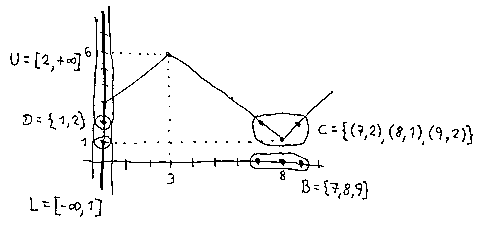
\includegraphics[width=11cm]{2021-1-C2/20210716_exercicio_7_figura.pdf}$$

\newpage


% «dois-jeitos-imagens»  (to ".dois-jeitos-imagens")
% (c2m211somas2p 20 "dois-jeitos-imagens")
% (c2m211somas2a    "dois-jeitos-imagens")

{\bf Dois jeitos de definir imagens de conjuntos}

Fazendo $B=\{7,8,9\}$ nas definições

do slide anterior obtemos:

$$\begin{array}{rcl}
  D  &=& \setofst {f(b)} {b∈\{7,8,9\}} \\
     &=& \{f(7), f(8), f(9)\} \\
     &=& \setofst {y∈\R} {y=f(7) ∨ y=f(8) ∨ y=f(9)} \\
     &=& \setofst {y∈\R} {∃x∈\{7,8,9\}.y=f(x)} \\
     &=& \setofst {d∈\R} {∃b∈\{7,8,9\}.d=f(b)} \\
     &=& D' \\
  \end{array}
$$

Isto vai valer para qualquer conjunto $B$, mesmo infinito.

\msk

Aplicação: digamos que duas pessoas estão tentando fazer o exercício

2b, e uma obteve $F([2,4)) = [5,6]$ e a outra obteve $F([2,4)) = (5,6]$.

Podemos testar se $5 ∈ \setofst{y∈\R}{∃x∈[2,4).f(x)=y} = F([2,4))$...


\newpage

% «sups-e-infs-em-portugues»  (to ".sups-e-infs-em-portugues")
% (c2m211somas2p 22 "sups-e-infs-em-portugues")
% (c2m211somas2a    "sups-e-infs-em-portugues")

{\bf Sups e infs em português}

Dá pra definir sups e infs em português se a gente usar dois truques:

1) ``$\R$ estendido'' vai ser $\Rest$,

2) ``acima'' e ``abaixo'' vão significar (temporariamente!) `$≥$' e `$≤$'.

\msk

Imagine que $a$ e $b$ são pontos do eixo $y$.

``$a$ está acima de $b$'' vai querer dizer `$a≥b$'.

``$a$ está estritamente acima de $b$'' vai querer dizer `$a>b$'.

Repare que cada ponto de $\R$ estendido está ``acima'' de si mesmo.

\msk

Idem pra ``abaixo'' e ``estritamente abaixo''.

\msk

O sup de um conjunto $D$ vai ser o ponto mais baixo dentre todos

os pontos que estão acima de todos os pontos de $D$.

\msk

O inf de um conjunto $D$ vai ser o ponto mais alto dentre todos

os pontos que estão abaixo de todos os pontos de $D$.

\newpage

% «exercicio-8»  (to ".exercicio-8")
% (c2m211somas2p 22 "exercicio-8")
% (c2m211somas2a    "exercicio-8")

{\bf Exercício 8.}

\ssk

Traduza para a linguagem do exercício 7:

\ssk

a) o ponto $P$ está acima de todos os pontos de $D$

b) o ponto $Q$ está acima de todos os pontos de $D$

c) o conjunto de todos os pontos de $\R$ estendido que estão

acima de todos os pontos de $D$

d) o conjunto de todos os pontos de $\R$ estendido que estão

abaixo de todos os pontos de $D$

e) o ponto mais baixo dentre todos os pontos de $\R$ estendido

que estão acima de todos os pontos de $D$

f) o ponto mais alto dentre todos os pontos de $\R$ estendido

que estão abaixo de todos os pontos de $D$

\newpage

% «exercicio-9»  (to ".exercicio-9")
% (c2m211somas2p 24 "exercicio-9")
% (c2m211somas2a    "exercicio-9")

{\bf Exercício 9.}

Digamos que:
%
$$\scalebox{0.9}{$
  \begin{array}{rcl}
  C  &=& \setofst {(b,f(b))} {b∈B}, \\
  D  &=& \setofst     {f(b)} {b∈B}, \\
  D' &=& \setofst {d∈\R} {∃b∈B.f(b)=d}, \\
  L  &=& \setofst {ℓ∈\R∪\{-∞,+∞\}} {∀d∈D.ℓ≤d}, \\
  U  &=& \setofst {u∈\R∪\{-∞,+∞\}} {∀d∈D.d≤u}, \\
  (β \text{ é o inf de } D) &=& (β∈L \text{ e } ∀α∈L.α≤β), \\
  (γ \text{ é o sup de } D) &=& (γ∈U \text{ e } ∀δ∈U.γ≤δ). \\
  \end{array}
  $}
$$

Dá pra calcular $L$, $U$, e o inf e o sup de $D$ só a partir do $D$...

então vamos ignorar os conjuntos $B$ e $C$ neste exercício.

\msk

a) Seja $D=(2,3)∪(4,5)$. Calcule $L$, $U$, $\inf D$, $\sup D$.

b) Seja $D=[2,3]∪[4,5]$. Calcule $L$, $U$, $\inf D$, $\sup D$.

c) Seja $D=\R$. Calcule $L$, $U$, $\inf D$, $\sup D$.

d) Seja $D=∅$. Calcule $L$, $U$, $\inf D$, $\sup D$.


\newpage

% «exercicio-10»  (to ".exercicio-10")
% (c2m211somas2p 25 "exercicio-10")
% (c2m211somas2a    "exercicio-10")

{\bf Exercício 10.}

\ssk

% (find-LATEX "edrxpict.lua" "beginpicture")

Lembre que:

\bsk

$f(x)=
    \unitlength=10pt
    \celllower=2.5pt%
    \def\cellfont{\scriptsize}%
    %
    \vcenter{\hbox{%
    \beginpicture(0,0)(11,7)
    \pictgrid%
    \pictpiecewise{(0,3)--(3,6)--(8,1)--(11,4)}%
    \put(3,6.5){\cell{(3,6)}}%
    \put(8,0.5){\cell{(8,1)}}%
    \pictaxes%
    \end{picture}%
    }}
   $

\bsk

a) Calcule $\sup(F([2,4]))$.

b) Calcule $\inf(F([2,4]))$.

c) Calcule $\sup(F([4,7]))$.

d) Calcule $\inf(F([4,7]))$.

e) Calcule $\sup(F([7,9]))$.

f) Calcule $\inf(F([7,9]))$.


\newpage

% «exercicio-11»  (to ".exercicio-11")
% (c2m211somas2p 26 "exercicio-11")
% (c2m211somas2a    "exercicio-11")

{\bf Exercício 11.}

\ssk

% (find-LATEX "edrxpict.lua" "beginpicture")

Lembre que:

\bsk

$f(x)=
    \unitlength=8pt
    \celllower=2.5pt%
    \def\cellfont{\scriptsize}%
    %
    \vcenter{\hbox{%
    \beginpicture(0,0)(11,7)
    \pictgrid%
    \pictpiecewise{(0,3)--(3,6)--(8,1)--(11,4)}%
    \put(3,6.5){\cell{(3,6)}}%
    \put(8,0.5){\cell{(8,1)}}%
    \pictaxes%
    \end{picture}%
    }}
   $

\bsk

Digamos que $P=\{ 1, 2,4, 5,6, 7,9, 10 \}$.

Represente graficamente \ColorRed{num gráfico só}:

\msk

a) $\sum_{i=1}^{N} \sup(F([a_i,b_i])) (b_i - a_i)$,

b) a curva $y=f(x)$,

c) $\sum_{i=1}^{N} \inf(F([a_i,b_i])) (b_i - a_i)$.

\msk

e verifique que você obteve algo bem parecido

com a figura do slide 2.



\newpage

% «metodos-nomes»  (to ".metodos-nomes")
% (c2m211somas2p 27 "metodos-nomes")
% (c2m211somas2a    "metodos-nomes")

{\bf Métodos de integração: nomes}

\def\sumiN#1{\sum_{i=1}^N #1 (b_i-a_i)}
\def\mname#1{\text{[#1]}}
%
$$\scalebox{0.95}{$
  \begin{array}{ccl}
  \mname{L}    &=& \sumiN {f(a_i)}                    \\[2pt]
  \mname{R}    &=& \sumiN {f(b_i)}                    \\[2pt]
  \mname{Trap} &=& \sumiN {\frac{f(a_i) + f(b_i)}{2}} \\[2pt]
  \mname{M}    &=& \sumiN {f(\frac{a_i+b_i}{2})}      \\[2pt]
  \mname{min}  &=& \sumiN {\min(f(a_i), f(b_i))}      \\[2pt]
  \mname{max}  &=& \sumiN {\max(f(a_i), f(b_i))}      \\[2pt]
  \mname{inf}  &=& \sumiN {\inf(F([a_i,b_i]))}        \\[2pt]
  \mname{sup}  &=& \sumiN {\sup(F([a_i,b_i]))}        \\
  \end{array}
  $}
$$

Cada uma dessas fórmulas é um ``método de integração''.

Todos esses ``métodos'' aparecem na página da Wikipedia,

mas com outros nomes e usando partições em que todos os

intervalos têm o mesmo comprimento.

\newpage

% «metodos-nomes-2»  (to ".metodos-nomes-2")
% (c2m211somas2p 27 "metodos-nomes-2")
% (c2m211somas2a    "metodos-nomes-2")

{\bf Métodos de integração: nomes (2)}

\ssk

Todas as fórmulas do slide anterior supõem que estamos

num contexto em que a partição $P$ está definida.

Se usamos elas com uma partição em subscrito,

como em $\mname{L}_{\{4,5,7\}}$, isso vai querer dizer

que a partição $P$ vai ser indicada no subscrito.

Por exemplo:
%
$$\scalebox{0.9}{$
  \begin{array}[t]{rcl}
  \mname{L}_{\{4,5,7\}} &=& \sumiN {f(a_i)} \\[5pt]
                        &=& f(a_1)(b_1-a_1) \\
                        &+& f(a_2)(b_2-a_2) \\[5pt]
                        &=& f(4)  (5-4) \\
                        &+& f(5)  (7-5,) \\
  \end{array}
  \quad
  \begin{array}[t]{rcl}
  \mname{L}_{\{6,7,8,9\}} &=& \sumiN {f(a_i)} \\[5pt]
                          &=& f(a_1)(b_1-a_1) \\
                          &+& f(a_2)(b_2-a_2) \\
                          &+& f(a_3)(b_3-a_2) \\[5pt]
                          &=& f(6)  (7-6) \\
                          &+& f(7)  (8-7) \\
                          &+& f(8)  (9-8). \\
  \end{array}
  $}
$$




\newpage

% «exercicio-12»  (to ".exercicio-12")
% (c2m211somas2p 29 "exercicio-12")
% (c2m211somas2a    "exercicio-12")

{\bf Exercício 12.}

\ssk

% (find-LATEX "edrxpict.lua" "beginpicture")

Lembre que:

\bsk

$f(x)=
    \unitlength=7pt
    \celllower=2.5pt%
    \def\cellfont{\scriptsize}%
    %
    \vcenter{\hbox{%
    \beginpicture(0,0)(11,7)
    \pictgrid%
    \pictpiecewise{(0,3)--(3,6)--(8,1)--(11,4)}%
    \put(3,6.5){\cell{(3,6)}}%
    \put(8,0.5){\cell{(8,1)}}%
    \pictaxes%
    \end{picture}%
    }}
   $

\bsk

Em cada um dos itens abaixo represente graficamente

num gráfico só a curva $y=f(x)$ e os dois somatórios pedidos.

a) $\mname{sup}_{\{1,10\}}$, 
   $\mname{inf}_{\{1,10\}}$

\ssk

b) $\mname{sup}_{\{1,2,5,6,9,10\}}$, 
   $\mname{inf}_{\{1,2,5,6,9,10\}}$

\ssk

c) $\mname{sup}_{\{1,2,4,5,6,7,9,10\}}$, 
   $\mname{inf}_{\{1,2,4,5,6,7,9,10\}}$

\bsk

d) $\mname{max}_{\{1,10\}}$, 
   $\mname{min}_{\{1,10\}}$

\ssk

e) $\mname{max}_{\{1,2,5,6,9,10\}}$, 
   $\mname{min}_{\{1,2,5,6,9,10\}}$



\newpage

% «exercicio-13»  (to ".exercicio-13")
% (c2m211somas2p 20 "exercicio-13")
% (c2m211somas2a    "exercicio-13")

{\bf Nossas partições preferidas}

Agora eu vou definir uma notação pra partição que

divide um intervalo em $N$ subintervalos iguais:
%
\def\baN{\frac{b-a}{N}}
%
$$
  \textstyle
  [a,b]_N = \{a, \; a+\baN, \; a+2\baN, \; \ldots, \; b\}
$$

\msk

{\bf Exercício 13.}

Calcule:

a) $[4,6]_1$

b) $[4,6]_{2^3}$

\msk

Dicas: $2^3=8$, e releia isto aqui:

\ssk

{\footnotesize

% (c2m211somas1p 16 "exercicio-9-dicas")
% (c2m211somas1a    "exercicio-9-dicas")
% http://angg.twu.net/LATEX/2021-1-C2-somas-1.pdf#page=16
\url{http://angg.twu.net/LATEX/2021-1-C2-somas-1.pdf\#page=16}

}

\bsk


Obs: mais tarde no curso você vai (ter que!)

aprender a fazer as suas próprias definições...

\newpage

% «exercicio-14»  (to ".exercicio-14")
% (c2m211somas2p 30 "exercicio-14")
% (c2m211somas2a    "exercicio-14")

{\bf Exercício 14.}

Lembre que:

\bsk

$f(x)=
    \unitlength=10pt
    \celllower=2.5pt%
    \def\cellfont{\scriptsize}%
    %
    \vcenter{\hbox{%
    \beginpicture(0,0)(11,7)
    \pictgrid%
    \pictpiecewise{(0,3)--(3,6)--(8,1)--(11,4)}%
    \put(3,6.5){\cell{(3,6)}}%
    \put(8,0.5){\cell{(8,1)}}%
    \pictaxes%
    \end{picture}%
    }}
   $

\bsk

Em cada um dos itens abaixo represente graficamente

num gráfico só a curva $y=f(x)$ e os dois somatórios pedidos.

a) $\mname{sup}_{[2,10]_{2^0}}$, 
   $\mname{inf}_{[2,10]_{2^0}}$

\ssk

b) $\mname{sup}_{[2,10]_{2^1}}$, 
   $\mname{inf}_{[2,10]_{2^1}}$

\ssk

c) $\mname{sup}_{[2,10]_{2^2}}$, 
   $\mname{inf}_{[2,10]_{2^2}}$

\ssk

d) $\mname{sup}_{[2,10]_{2^3}}$, 
   $\mname{inf}_{[2,10]_{2^3}}$


\newpage

{\bf Aproximações por cima}

Mais duas definições:

A melhor aproximação por cima para a integral de $f$

na partição $P$ é:
%
$$\Intover{P}{f(x)} = \mname{sup}_P,$$

O limite das aproximações por cima pra integral de $f$

no intervalo $[a,b]$ é:
%
$$\Intxover{a}{b}{f(x)} = \lim_{k→∞} \mname{sup}_{[a,b]_{2^k}},$$

Esse limite também é chamado de a ``integral por cima de $f$

no intervalo $[a,b]$''.


\newpage

{\bf Aproximações por baixo}

Mais duas definições:

A melhor aproximação por baixo para a integral de $f$

na partição $P$ é:
%
$$\Intunder{P}{f(x)} = \mname{inf}_P,$$

O limite das aproximações por baixo pra integral de $f$

no intervalo $[a,b]$ é:
%
$$\Intxunder{a}{b}{f(x)} = \lim_{k→∞} \mname{inf}_{[a,b]_{2^k}},$$

Esse limite também é chamado de a ``integral por baixo de $f$

no intervalo $[a,b]$''.


\newpage

% «definicao-integral»  (to ".definicao-integral")
% (c2m211somas2p 34 "definicao-integral")
% (c2m211somas2a    "definicao-integral")

{\bf A definição de integral}

\ssk

\def\eqa{\overset{\ColorRed{\Downarrow}}{=}}

A nossa definição de $\Intx{a}{b}{f(x)}$ vai ser:
%
$$\Intx     {a}{b}{f(x)} \;\;=\;\;
  \Intxover {a}{b}{f(x)} \;\; \eqa \;\;
  \Intxunder{a}{b}{f(x)}
$$

se a igualdade marcada com `$\eqa$' for verdade.

\msk
\msk

Se a igualdade `$\eqa$' for falsa vamos dizer que:

``$f(x)$ não é integrável no intervalo $[a,b]$'',

``$\Intx{a}{b}{f(x)}$ não está definida'', ou

``$\Intx{a}{b}{f(x)}$ dá erro''.

\msk
\msk

(Compare com $\frac{42}{0}$, que também ``não está definido'', ou ``dá erro''...)

\newpage

% «intoverunder»  (to ".intoverunder")
% (c2m211somas2p 35 "intoverunder")
% (c2m211somas2a    "intoverunder")
%
% «exercicio-15»  (to ".exercicio-15")
% (c2m211somas2p 35 "exercicio-15")
% (c2m211somas2a    "exercicio-15")

{\bf Como esses limites funcionam?}

Em Cálculo 1 você viu que algumas funções não são deriváveis.

Agora nós vamos ver que algumas funções não são integráveis.

O melhor modo de visualizar isso é usando estas definições:
%
$$\begin{array}{rcl}
  \D \Intoverunder{P}{f(x)} &=&
  \D \Intover     {P}{f(x)} -
     \Intunder    {P}{f(x)}
  \\[15pt]
  \D \Intxoverunder{a}{b}{f(x)} &=&
  \D \Intxover     {a}{b}{f(x)} -
     \Intxunder    {a}{b}{f(x)}
  \end{array}
$$

{\bf Exercício 15.}

\def\iou#1{\Intoverunder{[2,10]_{2^#1}}{f(x)}}

a) Verifique que no exercício 14 você desenhou $\iou0$,

$\iou1$, $\iou2$, e $\iou3$.

\msk

b) Calcule a área dessas quatro diferenças. \ColorRed{Veja o vídeo!}




\newpage

% «exercicio-16»  (to ".exercicio-16")
% (c2m211somas2p 36 "exercicio-16")
% (c2m211somas2a    "exercicio-16")

{\bf Exercício 16.}

Identifique nas figuras dos próximos dois slides:
%
\def\Io #1{\Intover      {[2,10]_{2^{#1}}} {f(x)}}
\def\Iu #1{\Intunder     {[2,10]_{2^{#1}}} {f(x)}}
\def\Iou#1{\Intoverunder {[2,10]_{2^{#1}}} {f(x)}}
%
$$\scalebox{0.9}{$
  \begin{array}{cccc}
  \Io1,  & \Io2,  & \Io3,  & \Io4, \\[10pt]
  \Iu1,  & \Iu2,  & \Iu3,  & \Iu4, \\[10pt]
  \Iou1, & \Iou2, & \Iou3, & \Iou4, \\[10pt]
  \end{array}
  $}
$$

$$%\scalebox{0.9}{$
  \Intx{2}{10}{f(x)}.
  %$}
$$

\msk

Dica: os ``$\Intoverunder{P}{\ldots}$''s são feitos de ``retângulos flutuando no ar'',

não de retângulos cujas bases estão em $y=0$.


\newpage

% «exercicio-16-defs»  (to ".exercicio-16-defs")
% (c2m211somas2p 37 "exercicio-16-defs")
% (c2m211somas2a    "exercicio-16-defs")
% (c2m211figsa    "defs-int")

% (find-LATEX "2021-1-C2-critical-points.lua" "Approxer-tests")
%L dofile     "2021-1-C2-critical-points.lua"
%L appr = Approxer {
%L     f      = f_do_slide_8,
%L     allcps = {3,8},
%L     a      = 2,
%L     b      = 10,
%L     N      = 4,
%L     method = "supin",
%L     what   = "ac",
%L   }
\pu

\long\def\ColorUpperA#1{{\color{red!20!white}#1}}
\long\def\ColorUpperB#1{{\color{Gold1!20!white}#1}}
\long\def\ColorUpperC#1{{\color{Green1!20!white}#1}}
\long\def\ColorUpperD#1{{\color{Blue1!20!white}#1}}
\long\def\ColorLowerA#1{{\color{red!80!white}#1}}
\long\def\ColorLowerB#1{{\color{Gold1!80!white}#1}}
\long\def\ColorLowerC#1{{\color{Green1!80!white}#1}}
\long\def\ColorLowerD#1{{\color{Blue1!80!white}#1}}
\long\def\ColorRealInt#1{{\color{Purple0!90!white}#1}}

\def\fwithapprs#1{%
  \vcenter{\hbox{%
    \beginpicture(0,0)(11,7)
    \pictgrid%
    #1%
    \pictpiecewise{(0,3)--(3,6)--(8,1)--(11,4)}%
    \pictaxes%
    \end{picture}%
  }}}

\def\UpperA{\ColorUpperA{\expr{appr:pict(2,  "supin", "c")}}}
\def\UpperB{\ColorUpperB{\expr{appr:pict(4,  "supin", "c")}}}
\def\UpperC{\ColorUpperC{\expr{appr:pict(8,  "supin", "c")}}}
\def\UpperD{\ColorUpperD{\expr{appr:pict(16, "supin", "c")}}}
\def\LowerD{\ColorLowerD{\expr{appr:pict(16, "infin", "c")}}}
\def\LowerC{\ColorLowerC{\expr{appr:pict(8,  "infin", "c")}}}
\def\LowerB{\ColorLowerB{\expr{appr:pict(4,  "infin", "c")}}}
\def\LowerA{\ColorLowerA{\expr{appr:pict(2,  "infin", "c")}}}

\def\fUpperA{\fwithapprs{\UpperA}}
\def\fUpperB{\fwithapprs{\UpperB}}
\def\fUpperC{\fwithapprs{\UpperC}}
\def\fUpperD{\fwithapprs{\UpperD}}
\def\fLowerA{\fwithapprs{\LowerA}}
\def\fLowerB{\fwithapprs{\LowerB}}
\def\fLowerC{\fwithapprs{\LowerC}}
\def\fLowerD{\fwithapprs{\LowerD}}
\def\fUpperLowerA{\fwithapprs{\UpperA\LowerA}}
\def\fUpperLowerB{\fwithapprs{\UpperB\LowerB}}
\def\fUpperLowerC{\fwithapprs{\UpperC\LowerC}}
\def\fUpperLowerD{\fwithapprs{\UpperD\LowerD}}
\def\fUpperLowerABCD{\fwithapprs{%
    \UpperA%
    \UpperB%
    \UpperC%
    \UpperD%
    \LowerD%
    \LowerC%
    \LowerB%
    \LowerA%
  }}
\def\fRealInt{\fwithapprs{\ColorRealInt{%
  \polygon*(2,0)(2,5)(3,6)(8,1)(10,3)(10,0)%
  }}}

% \newpage

% «exercicio-16-fig1»  (to ".exercicio-16-fig1")
% (c2m211somas2p 37 "exercicio-16-fig1")
% (c2m211somas2a    "exercicio-16-fig1")

\unitlength=6.5pt

$\fUpperLowerA
  \quad
  \fUpperLowerB
  \quad
  \fUpperLowerC
  \quad
  \fUpperLowerD
$

\bsk

\unitlength=20pt

$\fUpperLowerABCD
$

\newpage

% «exercicio-16-fig2»  (to ".exercicio-16-fig2")
% (c2m211somas2p 38 "exercicio-16-fig2")
% (c2m211somas2a    "exercicio-16-fig2")

\unitlength=5pt

$\begin{array}{ccccccccc}
 \fUpperA &≥& \fUpperB &≥& \fUpperC &≥& \ldots \\
                                 &&&&&& \rotl{≤} \\
                                 &&&&&& \fRealInt \\
                                 &&&&&& \rotl{≤} \\
 \fLowerA &≤& \fLowerB &≤& \fLowerC &≤& \ldots \\
 \end{array}
$


\newpage

% «exercicio-17»  (to ".exercicio-17")
% (c2m211somas2p 39 "exercicio-17")
% (c2m211somas2a    "exercicio-17")

{\bf Exercício 17: áreas no olhômetro}

A partir daqui eu vou supor que todo mundo sabe calcular

determinadas áreas ``no olho'' --- contando quadradinhos,

fazendo ``base $·$ altura'' (pra retângulos), ou

fazendo ``(base $·$ altura)/2'' (pra triângulos)...

\msk

Tente calcular a área da figura abaixo de cabeça.

%L pol = function (x,y,dx,dy)
%L     local x0, y0, x1, y1 = x,y,x+dx,y+dy
%L     return pformat("\\polygon*(%s,%s)(%s,%s)(%s,%s)(%s,%s)",
%L                    x0,y0, x0,y1, x1,y1, x1,y0)
%L   end
\pu
%
\unitlength=10pt
%
$$
  \vcenter{\hbox{%
    \beginpicture(0,0)(11,7)
    \pictgrid%
    \pictaxes%
    {%
     %\color{DarkGoldenrod1}%
     \color{DarkOrchid2}%
     \color{Honeydew4}%
     \color{Coral2}%
     \color{Orange1}%
     \expr{pol(2,3, 2,3)}%
     \polygon*(5,4)(5,6)(8,4)%
     \expr{pol(6.0,1.0, .5,.5)}%
     \expr{pol(6.5,1.5, .5,.5)}%
     \expr{pol(7.0,2.0, .5,.5)}%
     \expr{pol(7.5,2.5, .5,.5)}%
     \expr{pol(8.0,3.0, .5,.5)}%
     \expr{pol(8.5,3.5, .5,.5)}%
    }
    \end{picture}%
  }}
$$

\msk

Se você não conseguir \ColorRed{PEÇA AJUDA E DICAS

NO CANAL DO TELEGRAM URGENTE!!!!!!!!!!!!!!!}



\newpage

% «claramente-integravel»  (to ".claramente-integravel")
% (c2m211somas2p 39 "claramente-integravel")
% (c2m211somas2a    "claramente-integravel")

{\bf Funções ``claramente integráveis''}

Lembre que uma função $f(x)$ é integrável

entre $x=a$ e $x=b$ se e só se:

\def\Iou#1{\Intoverunder {[2,10]_{2^{#1}}} {f(x)}}
\def\Iou#1{\Intoverunder {[a, b]_{2^{#1}}} {f(x)}}

$$\lim_{k→∞} \left( \Iou{k} \right) = 0$$

Seja $d_k = \left( \Iou{k} \right)$; o `$d$' é de ``diferença''.

Cada $d_k$ pode ser interpretado de dois jeitos: como uma

figura feita de $2^k$ retângulos ``flutuando no ar'', ou

como a área total desses retângulos.


\newpage

% «claramente-integravel-2»  (to ".claramente-integravel-2")
% (c2m211somas2p 40 "claramente-integravel-2")
% (c2m211somas2a    "claramente-integravel-2")

{\bf Funções ``claramente integráveis'' (2)}

As primeiras 4 figuras do exercício 16 contêm

representações gráficas de $d_1$, $d_2$, $d_3$, $d_4$ --- 

são as áreas numa cor mais clara --- e se explicarmos

claramente pro leitor que é pra interpretar cada uma

daquelas figuras como a área da parte mais clara delas

nós podemos dizer que:
%
\unitlength=3.5pt
%
$$\begin{array}{rcl}
  (d_1, d_2, d_3, d_4, \ldots)
  &=& \left(\fUpperLowerA,
            \fUpperLowerB,
            \fUpperLowerC,
            \fUpperLowerD,
            \ldots
      \right)
  \\
  &=& (20, 14, 8, 4, \ldots)
  \\
  \end{array}
$$

E se o nosso leitor tiver prática suficiente ele vai

conseguir visualizar sozinho o que são $d_5, d_6, \ldots$

e ele vai conseguir \ColorRed{ver} que $\lim_{k→∞} d_k = 0$.

\newpage

% «claramente-integravel-3»  (to ".claramente-integravel-3")
% (c2m211somas2p 42 "claramente-integravel-3")
% (c2m211somas2a    "claramente-integravel-3")

{\bf Funções ``claramente integráveis'' (3)}

Alguns livros têm demonstrações completas de que

toda função $f:[a,b]→\R$ contínua é integrável ---

mesmo funções contínuas bem esquisitas, como essa aqui:

\ssk

{\footnotesize

\url{https://en.wikipedia.org/wiki/Weierstrass_function}

}

\msk

Essa demonstração é bem difícil --- mesmo o Pierluigi

Beneveri não faz ela inteira nas notas de aula dele...

A demonstração usa {\sl continuidade uniforme}:

\ssk

{\footnotesize

\url{https://en.wikipedia.org/wiki/Uniform_continuity}

}

\msk

...e a gente só entende as contas cheias de desigualdades

que aparecem na demonstração se a gente conseguir

visualizar o que cada somatório e cada desigualdade

dela ``quer dizer''... então vamos nos concentrar nas

visualizações, deixem as contas horríveis pra depois.

\newpage

% «claramente-integravel-p»  (to ".claramente-integravel-p")
% (c2m211somas2p 43 "claramente-integravel-p")
% (c2m211somas2a    "claramente-integravel-p")

{\bf Funções ``claramente integráveis'' (4)}

A nossa função preferida láááá do início do

curso --- que era $f(x) = 4 - (x-2)^2$ ---

é ``claramente integrável''...

% f = function (x) return 4 - (x-2)^2 end
% for x=0,4,0.25 do print(pformat("(%s,%s)", x, f(x))) end

%L f_parabola = function (x) return 4 - (x-2)^2 end
%L appr = Approxer {
%L     f      = f_parabola,
%L     allcps = {},
%L     a      = 0,
%L     b      = 4,
%L     N      = 4,
%L     method = "supin",
%L     what   = "ac",
%L   }
\pu

\def\fwithapprs#1{%
  \vcenter{\hbox{%
    \beginpicture(0,0)(4,4)
    \pictgrid%
    #1%
    \pictpiecewise{%
      (0,0)--%
      (0.25,0.938)--%
      (0.5,1.75)--%
      (0.75,2.438)--%
      (1,3)--%
      (1.25,3.438)--%
      (1.5,3.75)--%
      (1.75,3.938)--%
      (2,4)--%
      (2.25,3.938)--%
      (2.5,3.75)--%
      (2.75,3.438)--%
      (3,3)--%
      (3.25,2.438)--%
      (3.5,1.75)--%
      (3.75,0.938)--%
      (4,0)%
      }%
    \pictaxes%
    \end{picture}%
  }}}

Olhe pras figuras abaixo e convença-se

de que $\lim_{k→∞} d_k =0$:
%
\unitlength=12pt
%
$$\begin{array}{rcl}
  (d_2, d_3, d_4, \ldots)
  &=& \left(\fUpperLowerB,
            \fUpperLowerC,
            \fUpperLowerD,
            \ldots
      \right)
  \end{array}
$$

\bsk
\bsk

{\footnotesize

Truque: escolha um $d_k$. Todos os retângulos dele têm a

mesma largura; chame-a de $w$. A altura de cada retângulo

é no máximo $4w$ --- porque $∀x∈[0,4].|f'(x)|≤4$.

}

\newpage

% «funcoes-escada»  (to ".funcoes-escada")
% (c2m211somas2p 44 "funcoes-escada")
% (c2m211somas2a    "funcoes-escada")

{\bf Funções escada}

Uma {\sl função escada} é uma função definida por casos que é

constante em cada um dos casos, e em que todos os casos são

da forma ``$〈\textit{constante}〉 \text{ quando } x∈〈\textit{intervalo}〉$''. Por exemplo,
%
\unitlength=15pt
%
$$f(x) =
  \vcenter{\hbox{%
    \beginpicture(0,-2)(6,3)
    \pictgrid%
    \pictaxes%
    \pictpiecewise{(0,1)--(2,1)c (2,2)o-(3,2)o (3,-1)c (3,0)o--(4,0)c (4,2)o--(6,2)}%
    \end{picture}%
  }}
  =
  \scalebox{0.9}{$
  \begin{cases}
     1 & \text{quando $x∈(-∞,2]$}, \\
     2 & \text{quando $x∈(2,3)$}, \\
    -1 & \text{quando $x∈[3,3]$}, \\
     0 & \text{quando $x∈(3,4]$}, \\
     2 & \text{quando $x∈(4,+∞)$} \\
  \end{cases}
  $}
$$

Note que também poderíamos ter escrito

$x≤2$ ao invés de $x∈(-∞,2]$,

$x=3$ ao invés de $x∈[3,3]$, etc...

Ah, e o número de casos tem que ser {\sl finito}.


\newpage

% «exercicio-18»  (to ".exercicio-18")
% (c2m211somas2p 45 "exercicio-18")
% (c2m211somas2a    "exercicio-18")

{\bf Exercício 18.}

{\sl Toda função escada é integrável.}

Neste exercício você vai verificar os detalhes disto

só pra esta função escada bem simples:


\unitlength=15pt
%
$$f(x) =
  \vcenter{\hbox{%
    \beginpicture(0,0)(5,4)
    \pictgrid%
    \pictaxes%
    \pictpiecewise{(0,1)--(2,1)c (2,3)o-(5,3)}%
    \end{picture}%
  }}
  =
  \scalebox{1.0}{$
  \begin{cases}
     1 & \text{quando $x≤1$}, \\
     3 & \text{quando $1<x$} \\
  \end{cases}
  $}
$$

\def\Iou#1{\Intoverunder {[1,4]_{2^{#1}}} {f(x)}}

Seja $d_k = \Iou{k}$.

a) Represente graficamente $d_k$ para $k=0,1,2,3,4$.

b) Cada um destes `$d_k$'s tem exatamente um retângulo com

\phantom{b) }altura diferente de 0. Diga a largura e a altura dele.

c) Calcule $d_{10}$ (como um número).


\newpage

% «dirichlet»  (to ".dirichlet")
% (c2m211somas2p 46 "dirichlet")
% (c2m211somas2a    "dirichlet")

{\bf A função de Dirichlet}

A {\sl função de Dirichlet} é definida por:
%
$$f(x) =
  \begin{cases}
     0 & \text{quando $x∈\Q$}, \\
     1 & \text{quando $x∈\R∖\Q$} \\
  \end{cases}
$$

Ela não tem um nome oficial, então

vamos chamá-la de `$f$' nos próximos slides.

\msk

O gráfico dela alterna freneticamente entre $y=0$ e $y=1$.

\msk

Lembre que:

os números racionais são os cuja expansão decimal é

``periódica'', e os irracionais são os que não são assim;

entre cada dois racionais diferentes há um irracional, e

entre cada dois irracionais diferentes há um racional...

\newpage

% «dirichlet-2»  (to ".dirichlet-2")
% (c2m211somas2p 47 "dirichlet-2")
% (c2m211somas2a    "dirichlet-2")

{\bf A função de Dirichlet (2)}

\def\ui#1{\underline{#1}}

Lembre que podemos obter um irracional entre, digamos,

$a=\frac{10}{7}=1.42857\ui{142857}$ e
$b=\frac{1285715}{900000}=1.42857\ui{2}$,

modificando a expansão decimal de um dele e trocando-a

pela expansão decimal de $\sqrt{2}$ a partir de um

certo ponto... Por exemplo:

$$\begin{array}{rcl}
  \sqrt{2} &=& 1.41421356237... \\[5pt]
  b        &=& 1.42857\ui{222222}... \\
  c        &=& 1.42857156237... \\
  a        &=& 1.42857\ui{142857}... \\
  \end{array}
$$

Neste caso temos $a<c<b$, com $a,b∈\Q$ e $c∈\R∖\Q$.

Dá pra fazer algo parecido pra obter um racional

entre dois irracionais.


\newpage

% «dirichlet-3»  (to ".dirichlet-3")
% (c2m211somas2p 48 "dirichlet-3")
% (c2m211somas2a    "dirichlet-3")

{\bf A função de Dirichlet (3)}

Dá pra desenhar o gráfico da função de Dirichlet assim:
%
\unitlength=20pt
%
$$f(x) =
  \begin{cases}
     0 & \text{quando $x∈\Q$}, \\
     1 & \text{quando $x∈\R∖\Q$} \\
  \end{cases}
  \;\;
  =
  \;\;
  \vcenter{\hbox{%
    \beginpicture(0,0)(2,1)
    \pictgrid%
    \pictaxes%
    \pictpiecewise{(0.1,1)c (0.3,1)c (0.5,1)c (0.7,1)c (0.9,1)c
                   (1.1,1)c (1.3,1)c (1.5,1)c (1.7,1)c (1.9,1)c 
                   (0.0,0)c (0.2,0)c (0.4,0)c (0.6,0)c (0.8,0)c
                   (1.0,0)c (1.2,0)c (1.4,0)c (1.6,0)c (1.8,0)c (2.0,0)c 
                   }%
    \end{picture}%
  }}
$$

Repare que isso só funciona porque o desenho é claramente

ambíguo... um leitor ``normal'' não consegue descobrir no olho

quais são as coordenadas da bolinhas em $y=1$ e em $y=0$,

então ele é obrigado a olhar pra definição formal da $f(x)$...

\msk

e aí quando ele entende a definição formal da $f(x)$ ele

descobre que o desenho quer dizer ``muitas bolinhas em $y=1$,

muito próximas umas das outras, e muitas bolinhas em $y=0$

muito próximas das outras''...

\msk

...e ele entende que esse ``muitas'' quer dizer ``infinitas''.

% (sqrt 2)
% (/ 10.0 7) 
% (* (/ 1.0 7) 9999)
% (* 1.428572222 900000)
% (/ 1285715 900000.0)



\newpage

% «exercicio-19»  (to ".exercicio-19")
% (c2m211somas2p 49 "exercicio-19")
% (c2m211somas2a    "exercicio-19")

{\bf Exercício 19.}

A função de Dirichlet é um dos exemplos mais simples

de uma função que não é integrável.

\msk

\def\Iou#1{\Intoverunder {[0,1]_{2^{#1}}} {f(x)}}

Sejam $f(x)$ a função de Dirichlet,

e $d_k = \Iou{k}$.

\msk

a) Represente graficamente $d_0, d_1, d_2, d_3$.

b) Calcule no olhômetro o limite $\lim_{k→∞} d_k$.

\phantom{b)} (Dica: esse limite não dá zero...)

\msk

c) Represente graficamente
$\mname{max}_{[0,1]_{2^2}}$ e
$\mname{min}_{[0,1]_{2^2}}$.

(Dica: o método do máximo ``não enxerga'' os pontos

com $y=1$...) 


\newpage

% «trailer»  (to ".trailer")
% (c2m211somas2p 50 "trailer")
% (c2m211somas2a    "trailer")
% Questão:  (c2m202p1p 3 "questao-1")
%           (c2m202p1a   "questao-1")
% Gabarito: (c2m202p1p 8 "gabarito-1")
%           (c2m202p1a   "gabarito-1")

{\bf Propriedades da integral: trailer}

No próximo PDF nós vamos começar a ver as propriedades da integral ---
ou, mais precisamente, as propriedades da operação $\Intx{a}{b}{f(x)}$
que nós definimos como um limite complicado. Nós vamos ver 1) que ela
realmente calcula áreas, 2) que \ColorRed{em certas situações}
``integrar'' e ``derivar'' são operações inversas uma da outra, 3) que
\ColorRed{em certas situações} podemos usar ``antiderivadas'' pra
calcular integrais bem rápido.

No semestre passado metade dos alunos não entenderam nada disso, e
numa questão em que eu pedia pra eles calcularem a área dessa figura
aqui de dois jeitos diferentes eles concluiram que a área dessa figura
era 4...
%
\unitlength=10pt
%
$$
  \vcenter{\hbox{%
    \beginpicture(0,0)(3,3)
    \pictgrid%
    \pictaxes%
    {%
     %\color{DarkGoldenrod1}%
     %\color{DarkOrchid2}%
     %\color{Honeydew4}%
     %\color{Coral2}%
     \color{Orange1}%
     \polygon*(0,0)(0,1)(1,1)(1,2)(2,2)(2,0)(0,0)%
    }
    \end{picture}%
  }}
$$
%

\ColorRed{Não seja como eles.}



% (find-booksfile "__analysis/__analysis.el" "beneveri")










\GenericWarning{Success:}{Success!!!}  % Used by `M-x cv'

\end{document}

%  ____  _             _         
% |  _ \(_)_   ___   _(_)_______ 
% | | | | \ \ / / | | | |_  / _ \
% | |_| | |\ V /| |_| | |/ /  __/
% |____// | \_/  \__,_|_/___\___|
%     |__/                       
%
% «djvuize»  (to ".djvuize")
% (find-LATEXgrep "grep --color -nH --null -e djvuize 2020-1*.tex")

 (eepitch-shell)
 (eepitch-kill)
 (eepitch-shell)
# (find-fline "~/2021.1-C2/")
# (find-fline "~/LATEX/2021-1-C2/")
# (find-fline "~/bin/djvuize")

cd /tmp/
for i in *.jpg; do echo f $(basename $i .jpg); done

f () { rm -fv $1.png $1.pdf; djvuize $1.pdf }
f () { rm -fv $1.png $1.pdf; djvuize WHITEBOARDOPTS="-m 1.0" $1.pdf; xpdf $1.pdf }
f () { rm -fv $1.png $1.pdf; djvuize WHITEBOARDOPTS="-m 0.5" $1.pdf; xpdf $1.pdf }
f () { rm -fv $1.png $1.pdf; djvuize WHITEBOARDOPTS="-m 0.25" $1.pdf; xpdf $1.pdf }
f () { cp -fv $1.png $1.pdf       ~/2021.1-C2/
       cp -fv        $1.pdf ~/LATEX/2021-1-C2/
       cat <<%%%
% (find-latexscan-links "C2" "$1")
%%%
}

f 20210716_exercicio_7_figura

f 20201213_area_em_funcao_de_theta
f 20201213_area_em_funcao_de_x
f 20201213_area_fatias_pizza



%  __  __       _        
% |  \/  | __ _| | _____ 
% | |\/| |/ _` | |/ / _ \
% | |  | | (_| |   <  __/
% |_|  |_|\__,_|_|\_\___|
%                        
% <make>

 (eepitch-shell)
 (eepitch-kill)
 (eepitch-shell)
# (find-LATEXfile "2019planar-has-1.mk")
make -f 2019.mk STEM=2021-1-C2-somas-2 veryclean
make -f 2019.mk STEM=2021-1-C2-somas-2 pdf

% Local Variables:
% coding: utf-8-unix
% ee-tla: "c2so2"
% ee-tla: "c2m211somas2"
% End:
